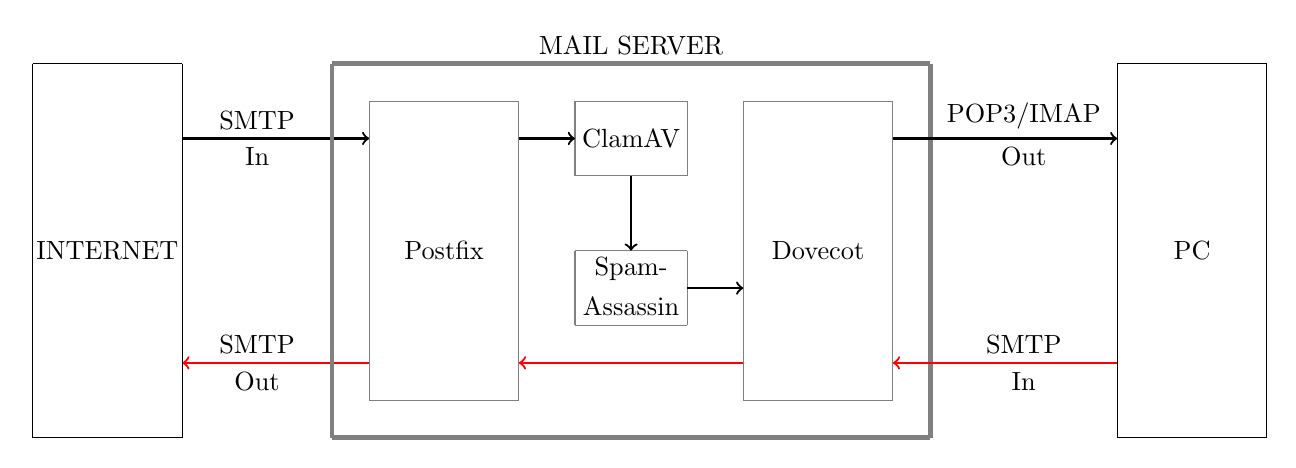
\begin{tikzpicture}[scale=0.95, every node/.style={scale=0.95}]

%SMTP-OUT arrow
\draw [red, thick, <-] (0,1) -- (2.5,1);
\node [above] at (1,1) {SMTP};
\node [below] at (1,1) {Out};

%SMTP-IN arrow
\draw [thick, ->] (0,4) -- (2.5,4);
\node [above] at (1,4) {SMTP};
\node [below] at (1,4) {In};

%Large Server Box
\draw [ultra thick, gray] (2,0) -- (10,0);
\draw [ultra thick, gray] (2,0) -- (2,5);
\draw [ultra thick, gray] (2,5) -- (10,5);
\draw [ultra thick, gray] (10,5) -- (10,0);

%Client-Side Arrows and Labels

\draw [thick, ->] (9.5,4) -- (12.5,4);
\draw [red, thick, <-] (9.5,1) -- (12.5,1);

\node [above] at (11.25,4) {POP3/IMAP};
\node [below] at (11.25,4) {Out};

\node [above] at (11.25,1) {SMTP};
\node [below] at (11.25,1) {In};

%PC Box

\draw (12.5,0) -- (12.5,5);
\draw (12.5,5) -- (14.5,5);
\draw (14.5,0) -- (14.5,5);
\draw (12.5,0) -- (14.5,0);

%Internet Box

\draw (0,0) -- (0,5);
\draw (0,5) -- (-2,5);
\draw (-2,5) -- (-2,0);
\draw (-2,0) -- (0,0);

%Box Labels
\node at (13.5,2.5) {PC};
\node at (-1,2.5) {INTERNET};
\node [above] at (6,5) {MAIL SERVER};

%Postfix box and label

\draw [gray] (2.5,0.5) -- (2.5,4.5);
\draw [gray] (2.5,0.5) -- (4.5,0.5);
\draw [gray] (2.5,4.5) -- (4.5,4.5);
\draw [gray] (4.5,4.5) -- (4.5,0.5);
\node at (3.5,2.5) {Postfix};

%Dovecot Box

\draw [gray] (7.5,0.5) -- (7.5,4.5);
\draw [gray] (7.5,0.5) -- (9.5,0.5);
\draw [gray] (7.5,4.5) -- (9.5,4.5);
\draw [gray] (9.5,4.5) -- (9.5,0.5);
\node at (8.5,2.5) {Dovecot};

%Supplementerys Box and labels

\draw [gray] (5.25,4.5) -- (6.75,4.5);
\draw [gray] (5.25,3.5) -- (5.25,4.5);
\draw [gray] (6.75,4.5) -- (6.75,3.5);
\draw [gray] (6.75,3.5) -- (5.25,3.5);
\node at (6,4) {ClamAV};

\draw [gray] (5.25,2.5) -- (6.75,2.5);
\draw [gray] (5.25,1.5) -- (5.25,2.5);
\draw [gray] (6.75,2.5) -- (6.75,1.5);
\draw [gray] (6.75,1.5) -- (5.25,1.5);
\node at (6,2.25) {Spam-};
\node at (6,1.75) {Assassin};

%Internal Arrows

\draw [thick, ->] (4.5,4) -- (5.25,4);
\draw [thick, ->] (6,3.5) -- (6,2.5);
\draw [thick, ->] (6.75,2) -- (7.5,2);

\draw [red, thick, <-] (4.5,1) -- (7.5,1);

\end{tikzpicture}